\chapter{État de l'Art: Simulation Multi-Agents et Répartition des Tâches}
\label{ChapitreEASMA}

	Afin de comprendre et reproduire les capacités complexes des insectes sociaux, ceux-ci sont étudiés depuis une cinquantaine d'années dans le domaine des Simulations Multi-Agents (SMA). Plusieurs travaux ont ainsi pu reproduire et approcher leurs capacités d'auto-organisation dynamique par la simulation, notamment Swarm Intelligence \cite{bonabeau_natural_1999} et bien d'autres \cite{drogoul_simulation_1993, schmickl_taskselsim_2008, dornhaus_task_1998}. La répartition du travail, ou allocation des tâches est au cœur de ces problématiques. Ce chapitre présente quelques modèles théoriques présents dans la littérature ainsi que quelques applications de ces derniers, notamment dans le cadre de la simulation d'insectes sociaux.
	
    \subsubsection*{Modèles Mathématiques}
		Bien que nous parlions ici de simulations multi-agents, il est tout de même intéressant d'en observer leurs principales alternatives, les modèles mathématiques. Souvent à base d'équations différentielles, ces modèles permettent de rendre compte d'évolution de populations par rapport à des paramètres de haut niveau. Un des premiers et des plus cités est le système d'équations "Proies-Prédateurs" de V.Volterra \cite{volterra_variations_1928}. Celui-ci reproduit les fluctuations de deux populations, l'une se nourrissant de l'autre, au travers de deux équations différentielles inter-connectées prenant la forme :
		
		\begin{equation}
  			\left\{\begin{array}{@{}l@{}}
    			\frac{dN_1}{dt}=(\epsilon_1-\gamma_1 N_2) N_1\\
      			\frac{dN_2}{dt}=(- \epsilon_2 + \gamma_2 N_1) N_2
  			\end{array}\right.\,
		\end{equation}
		
		\begin{figure}
		\centering
		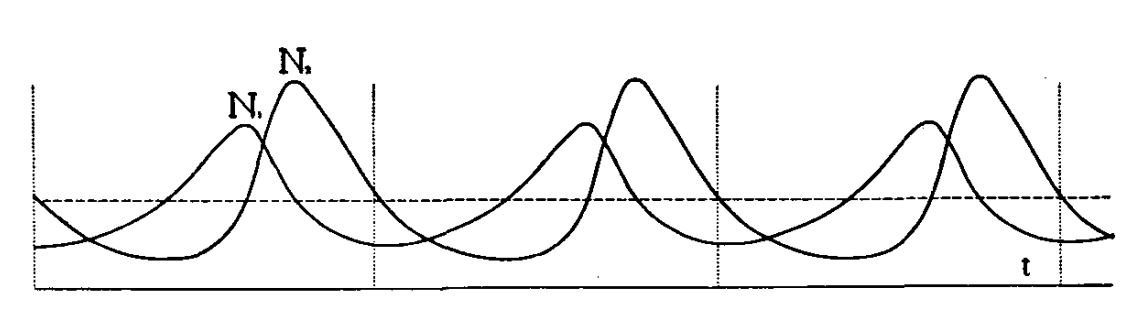
\includegraphics[width=0.9\textwidth]{./Pictures/Graphs/Volterra.JPG}
		\caption{D'après les travaux de V. Volterra\cite{volterra_variations_1928}. Évolution des populations du système mathématique "Proies-Prédateurs", avec $N_2$ écrit en haut et $N_1$ dessous.}
		\label{volterra}
		\end{figure}
		
		avec $N_1$ et $N_2$ les populations des deux espèces en nombre d'individus, respectivement les proies et les prédateurs. $\epsilon_1$ représente le taux de croissance des proies en l'absence de prédateur, et $\epsilon_2$ le taux de décroissance des prédateurs en l'absence de proie. Ensuite, $\gamma_1$ représente l'efficacité de chasse des prédateurs ainsi que l'efficacité de fuite des proies, là où $\gamma_2$ peut représenter l'efficacité des prédateurs à convertir les proies en descendance, ce qui peut revenir au même. $\frac{dN_1}{dt}$ représente les variations de la population des proies au cours du temps, et $\frac{dN_2}{dt}$ celles des prédateurs. La Figure \ref{volterra} est tirée des travaux de V.Volterra et illustre ce système d'équations en fonction du temps, pour des paramètres choisi par l'auteur. Nous allons décrire ces équations, en prenant l'exemple classique d'une population de loups $N_2$ confrontée à une population de moutons $N_1$. Plus les loups sont nombreux ($N2$ est grand) plus les moutons se font chasser : $\gamma_1 N_2$ est élevé, la croissance de $N1$ est alors diminuée car $\epsilon_1$ devient de plus en plus faible par rapport à $\gamma_1 N_2$. La population de moutons commence même à diminuer lorsque $\gamma_1 N_2$ devient supérieur à $\epsilon_1$, car $N1$ est alors multiplié par un nombre négatif (puisque $\epsilon_1 < \gamma_1 N_2$). La variation de population de moutons au cours du temps $\frac{dN_1}{dt}$ est alors négative, ce qui veut mathématiquement dire que la population de moutons diminue. Arrivé à un certain point, il n'y a plus assez de moutons pour la population de loups qui commence alors à s'effondrer : $-\epsilon_2 > \gamma_2 N_1$, donc $\frac{dN_2}{dt}$ est négative. Peu après, la faible population de loups transforme l'environnement en un paradis pour moutons qui voient alors leur population grimper, $\gamma_1 N_2$ étant très faible, le coefficient de $N_1$ est proche de $\epsilon_1$, la variation de population de moutons est alors proche de son maximum. Cela transforme peu après l'environnement en un paradis pour loups rempli de moutons, $\gamma_2 N_1$ est élevé, $- \epsilon_2 + \gamma_2 N_1$ et du même coup $\frac{dN_2}{dt}$ sont alors proches de leur maximum, la population de loup augmente rapidement. Ensuite, tout recommence de manière cyclique, ce que nous retrouvons dans la Figure \ref{volterra}.
		
		Certains modèles mathématiques ont été créés pour simuler différents aspects de colonies d'abeilles. Par exemple, le modèle HoPoMo \cite{schmickl_hopomo_2007} simule une version simplifiée de répartition des tâches et se concentre sur les ressources de la colonie. S. C. Pratt \cite{pratt_optimal_1999} s'est intéressé à la prise de décision de la colonie quant à la construction de nouvelles cellules pour y stocker le nectar. M. A. Becher et al. \cite{becher_brood_2010} se sont intéressés à l'impact de variation de température au niveau de couvain sur le butinage de ces abeilles une fois devenues adultes. La modèle BEEHAVE \cite{becher_beehave_2014} utilise un système d'équations différentielles pour décrire la colonie à l'intérieur de la ruche, populations, nourriture, couvain, Varroa, mais un système multi-agent pour décrire le butinage.
		
		Bien qu'efficace, ce genre de simulation présente quelques lacunes \cite{drogoul_multi-agent_1992}. Se focalisant sur les populations, ils ne rendent pas compte des décisions prises par chaque individu, ni de leurs stratégies ou comportements. Il est de ce fait impossible pour ces simulations de prendre en compte l'importance de différents stimulus pour la réalisation de certaines actions. De la même manière, les contacts et interactions entre individus ne sont pas simulées. Les populations n'altèrent pas leur environnement, leurs actions sont seulement vues d'une manière probabiliste, et seuls leurs résultats sont pris en compte. De plus, les modélisations mathématiques font apparaitre des paramètres n'ayant pas vraiment de sens du point de vue du système réel, un peu à la manière des $\gamma_1$ et $\gamma_2$ de Volterra, dans son exemple pourtant très simple. Ces points nous font nous tourner vers la simulation multi-agents afin de représenter le système complexe qu'est la colonie d'abeilles, fondamentalement dépendant des interactions et contacts entre individus.
			
			
	\section{Modèles existants de répartition des tâches}
	La division du travail, concept découlant de l'auto-organisation \cite{labella_division_2006}, se produit lorsque plusieurs agents décident quelle tâche exécuter parmi un ensemble de travaux à réaliser dans un environnement partagé. Les sociétés d'individus doivent trouver des moyens de répartir efficacement leur main-d'œuvre entre les tâches nécessaires pour survivre et s'étendre. En informatique, le contrôle décentralisé inspiré par les insectes sociaux a été étudié pendant des années et s'est avéré efficace dans de nombreuses applications. Dans cette section, nous allons passer en revue ce qui a été fait dans le domaine des modèles de répartition des tâches.
	
	
		\subsection{Foraging For Work}
        Dans ce modèle, les différentes tâches que les agents doivent accomplir sont spatialement dispersées en zones \cite{franks_foraging_1994}. Les agents, en recherche active de travail, tentent d'exécuter la tâche associée à leur zone. Les zones offrent une quantité fixe de travail : lorsque suffisamment d'agents y travaillent, aucun agent supplémentaire ne pourra effectuer cette tâche. Ceux-ci vont alors exécuter un déplacement aléatoire. Ainsi, les zones surpeuplées "poussent" indirectement les agents vers les zones voisines, ce qui entraîne une division du travail. Lorsque de nouveaux agents apparaissent dans une zone spécifique et que les agents meurent de vieillesse, ce modèle assez simple recrée le polyéthisme d'âges : les agents du même âge effectuent globalement les mêmes tâches, que nous retrouvons dans les colonies d'abeilles \cite{seeley_age_1991}. En effet, la zone voyant des agents naitre va contenir plus d'agents qu'elle n'offre de travail, là où une zone voyant des agents mourir aura plus de travail à offrir qu'elle ne contient d'agents. Ainsi, nous obtenons une zone de naissance qui aura tendance à repousser les agents, que la zone de "mort" va alors capter, ayant besoin de main d'œuvre. Nous obtenons une répartition spatiale liée à l'âge des individus, et ainsi une forme de polyéthisme d'âge car les zones sont associées à des tâches. Ce modèle nous intéresse particulièrement pour cette capacité. En effet chez les abeilles domestiques, une hypothèse est que la migration des nourrices vers le rôle de butineuse est provoquée par l'émergence de nouvelles nourrices au centre de zones de couvain  \cite{seeley_age_1991}. Ainsi, les jeunes nourrices repoussent les plus âgées vers d'autres activités, ce que le \textit{Foraging For Work} est tout à fait à même de recréer.
        
        Pour résumer, ce modèle repose sur deux hypothèses fortes :
        
        1. Chaque tâche est associée à un niveau de priorité, connu de tous les agents.
        
        2. Les tâches sont dispersées en zones géographiques définies.
        
        
		\subsection{Modèles à Seuils}
		\label{subsectionRTM}
		\subsubsection{FTM : "Fixed Threshold Model" \cite{bonabeau_natural_1999}}
        Avec ce modèle, chaque tâche a un score, représentant sa priorité. La probabilité qu'un agent s'engage dans une tâche est directement proportionnelle à son score. Le FTM est basé sur trois hypothèses fondatrices, dont voici la première : chaque tâche est associée à un stimulus. Le score de chaque tâche est calculé à partir de l'intensité du stimulus associé perçu par l'agent, généralement à l'aide d'une fonction sigmoïde. Soit $T$ la tâche évaluée par l'agent, $P(T)$ le score de la tâche $T$ et $S_T$ son stimulus associé (simple ou complexe) perçu par l'agent, ces fonctions prennent alors la forme :
			
\begin{equation}
\label{equationSigmoid}
	P(T) = \frac{S_T^n}{S_T^n + \Theta_T^n} \;\;\; ou \;\;\; P(T) = 1 - \frac{S_T^n}{S_T^n + \Theta_T^n}
\end{equation}	
 avec $n$ un entier pour la non-linéarité de la fonction (généralement $n=2$ \cite{schmickl_taskselsim_2008, gautrais_emergent_2002}) et $\Theta_T$ le seuil de la tâche, aussi appelé biais, de la sigmoïde. La Figure \ref{sigmoids} présente différentes sigmoïdes mettant en valeur l'impact du paramètre $\Theta_T$, propre à chaque agent. Le seuil sert en quelque sorte de point d'ancrage : lorsque le seuil est strictement équivalent au stimulus d'entrée, alors la valeur du résultat est exactement $\frac{1}{2}$. Ce biais est utilisé pour modifier la perception des agents : avec un biais très faible, les agents sont très sensibles au stimulus associé et s'engagent dans la tâche plus tôt que les agents avec un biais plus élevé \cite{dornhaus_task_1998}. 
		
		\begin{figure}
		\centering
		\includegraphics[width=0.5\textwidth]{./Pictures/Figures/sigmoids.png}
		\caption{L'influence du paramètre thêta ($\Theta$) sur la forme des sigmoides.}
		\label{sigmoids}
		\end{figure}
        
        Largement utilisés pour modéliser et piloter des simulations d'insectes sociaux (voir section \ref{sectionAppli}), les modèles à seuils reposent fortement sur l'association entre tâches et stimulus. Les modèles à seuils supposent également que l'exécution d'une tâche diminue le stimulus qui lui est associé, et que ne pas exécuter une tâche augmente son stimulus associé. Le stimulus doit être une représentation de la priorité de la tâche qui lui est associée, à tout moment. 
        
        Par exemple, Bonabeau et. al. \cite{bonabeau_quantitative_1996} utilisèrent un FTM pour modéliser la répartition du travail au sein d'une espèce de fourmi contenant deux types d'individu aux caractéristiques physiques très différentes \cite{wilson_relation_1984}. Appelés "Majors" et "Minors" dans leurs travaux, ces castes correspondent respectivement à ce que nous pourrions voir comme de grands soldats et de petites ouvrières. Dans la nature, il a été observé que les ouvrières travaillent en permanence, alors que les soldats travaillent seulement lorsque la demande est trop forte par rapport au nombre d'ouvrières présentes. Ces deux castes ont alors été modélisées, chacune avec un seuil différent pour une même tâche abstraite. 
        Les ouvrières ont reçu un seuil très faible, elles s'engagent donc dans la tâche même lorsque le stimulus déclencheur est relativement faible. À l'inverse, les soldats ont un seuil élevé, elles nécessitent donc un stimulus déclencheur très intense pour engager la tâche. Ainsi, lorsque le nombre d'ouvrières est suffisant pour maintenir le stimulus à un niveau faible (elles sont suffisamment nombreuses par rapport à la demande), les soldats ne travaillent pas car le stimulus n'atteindra jamais une valeur suffisamment élevée. Lorsque des ouvrières sont retirées de la simulation (ou de la colonie), le reste des ouvrières ne parvient plus à maintenir le stimulus bas : la demande dépasse l'offre. Le stimulus grimpe donc régulièrement, jusqu'à atteindre le seuil déclencheur des soldats, qui se mettent alors au travail. Lors de la réintroduction des ouvrières, les soldats arrêterons rapidement de travailler, le stimulus déclencheur redevenant trop faible du fait du travail des nouvelles ouvrières. On obtient donc un exemple d'auto-organisation sans aucun contrôle central, sur une seule tâche et avec deux populations aux seuils fixes, mais différents.
		
		Dans ce modèle, chaque tâche a une probabilité d'interruption aléatoire évaluée à chaque pas de temps \cite{gautrais_emergent_2002}. Dès lors, l'agent recherche une nouvelle tâche en utilisant les scores de chaque tâche. Cette interruption aléatoire repose sur une hypothèse : le score représente directement la priorité de la tâche. Ainsi, en interrompant régulièrement l'agent, on le force à observer ces niveaux de priorité, nous assurant ainsi qu'il exécute toujours la tâche la plus prioritaire.
        
        \subsubsection{RTM : "Response Threshold Model", Renforcement du biais}
        Sur la base du FTM et de l'équation \ref{equationSigmoid}, différents travaux des années 90 \cite{theraulaz_response_1998,carbonell_multi-agent_1994, gautrais_emergent_2002} ont proposé de mettre en place des mécanismes de renforcement de la valeur $\Theta$. Modifier ainsi la sensibilité des agents pendant l'exécution offre la possibilité de former des spécialistes. Cette mise à niveau du FTM est plus généralement appelée "Response Threshold Model".
        
        Cicirello et Smith \cite{cicirello_wasp-like_2004} utilisèrent un modèle à seuils pour résoudre un problème d'allocation de ressource : une ligne d'assemblage de \textit{General Motors} qui doit peindre de différentes couleurs des camions tout juste assemblés. Chaque compartiment de peinture est alors vu comme un agent qui possède une tâche par couleur de camion. Ainsi, une tâche consiste à peindre un camion d'une couleur, et changer de couleur signifie changer de tâche. Chaque tâche possède un seuil variable, permettant d'exprimer à la fois la spécialisation d'un compartiment pour une couleur, mais aussi indirectement d'exprimer le coût du changement de couleur. En effet, lors d'un changement de couleur, beaucoup de temps est perdu car il faut purger tout le système du compartiment, gâchant du même coup une bonne quantité de peinture. L'idée est donc de minimiser les coûts en peinture ainsi que le temps pour peindre une grande série de camions de couleurs différentes et inconnues \textit{a priori}. Une file de camions à peindre arrive en entrée et les compartiments doivent en accepter certains pour les peindre. Un compartiment ajuste les seuils de ses tâches à chaque pas de temps. Ainsi, il diminue celui de sa tâche correspondant à sa couleur actuelle, augmentant ses chances d'accepter de peindre un camion de sa couleur. À l'inverse, il augmente les seuils de toutes ses autres tâches. Lorsqu'un compartiment n'a aucun camion à peindre, il diminue alors tous ses seuils de manière exponentielle.
        
        De cette manière, Cicirello et Smith arrivent à grandement limiter le nombre de changement de couleurs nécessaires, tout en conservant un rendement proche des méthodes traditionnellement utilisées pour cette classe de problème.
        
        
        \section{Applications de Modèles de Répartitions des Tâches}
        \label{sectionAppli}
        Nous nous intéressons ici à quelques applications pratiques de modèles théoriques, notamment ceux que nous venons de décrire. 
        
        \paragraph{}
        Dans ses travaux, Brian R. Johnson \cite{johnson_division_2010} propose un modèle de répartition des tâches décrivant les comportements et physiologies d'ouvrières d'une colonie d'abeilles. Directement inspiré d'observations réelles, il propose de séparer la vie d'une ouvrière en quatre étapes : très jeune, nourrice, "age moyen", butineuse. 
        
        Après émergence, une ouvrière "très jeune" n'est pas tout à fait prête, ainsi elle termine son développement pendant environ une semaine. Pendant ce temps elle se nourrie de pollen et nettoie les cellules. Elle devient ensuite systématiquement une nourrice. 
        
        Les nourrices se chargent majoritairement des soins au couvain. À l'instar du modèle "Foraging for Work", les abeilles naissantes viennent prendre la place de ces nourrices, qui sont progressivement poussée en dehors de la zone du couvain. Ainsi éloignées, ces nourrices sont alors moins sujettes aux phéromones de la reine et du couvain, qui cessent alors d'altérer leur développement. Elles deviennent alors des abeilles d'âge moyen. Il est alors intéressant de constater que cet "âge moyen" n'est en réalité pas lié à un âge. Une abeille qui parviendrait à ne pas se faire pousser hors de la zone du couvain pourrait ainsi rester théoriquement nourrice toute sa vie. L'auteur présente l'exemple d'une expérimentation réalisée par des biologistes, où les abeilles naissantes sont retirées de la colonie. Les nourrices n'étaient alors pas poussées et ont bien été observées continuer cette activité.
        
        La phase d'âge moyen est décrite comme une succession de changements, un état transitoire. L'abeille y effectue différentes tâches. L'auteur propose de séparer cette phase en deux sous parties successives. Une abeilles nouvellement arrivée dans cette phase effectuera des tâches d'entretiens du nid (nettoyage, réparation, construction) aux alentours des zones de couvains, se superposant donc spatialement aux nourrices. Pendant ce temps sa physiologie change, différentes hormones et phéromones s'influent mutuellement pour guider la modification. l'Hormone Juvénile (HJ) est centrale dans ce processus. Avec son HJ grandissante, l'abeille ira se placer de plus en plus proche de la sortie de la ruche, en effectuant notamment la tâche de receveuse. Par la suite, elle deviendra physiologiquement apte à butiner. À ce point de développement, l'abeille partira butiner dès qu'elle suivra une danse de recrutement par une autre butineuse, ou qu'elle ne parviendra plus à trouver de travail en tant que receveuse.
        
        Les butineuses ne réalisent plus aucune tâche à l'intérieur du nid. Elles ramène eau, cire, pollen et nectar à la colonie. Les butineuses ne semblent pas se spécialiser dans une quelconque ressource. Les butineuses, via les receveuses, répandent une hormone/phéromone à effet inhibiteur dans la colonie, ralentissant le développement d'autres abeilles en butineuses.
        
        L'auteur récapitule aussi ce que nous savons actuellement des abeilles d'hiver, ressemblant à un état de nourrice prolongé, mais semblant être décoléré de toute répartition du travail. En hiver, toutes les abeilles partagent cette physiologie. Peu d'information sont présentes sur ce sujet dans la littérature, mais quelques études montrent que le faible niveau de pollen réduit fortement la capacité de la colonie à élever des larves. Ainsi, une colonie sans larves transitionnerait automatiquement vers un état hivernal. Ensuite, le modèle présenté n'explique pas le retour à la physiologie de nourrice que réalisent certaines butineuses. L'auteur cite même quelques expérimentations montrant que près de 20\% des butineuses redeviennent nourrices en quelques jours (même en l'absence de couvain \cite{huang_regulation_1996}).
        
        L'auteur en profite pour souligner le peu de recherches réalisées sur les abeilles "d'âge moyen", car elles jouent un rôle clé dans la répartition du travail au sein de la colonie.
        
        \paragraph{}
        Drogoul et.al. \cite{drogoul_multi-agent_1992} ont réalisé une simulation multi-agents de colonie de fourmis, ainsi qu'un modèle de tâche et de sélection de tâches. Ils ne parlaient à l'époque (1992) pas encore de systèmes à seuils, mais en étaient déjà très proches. Dans leur modèle, chaque tâche est liée à un stimulus déclencheur, et possède un poids. Pour être sélectionnée, la tâche doit multiplier son poids et son stimulus déclencheur, et comparer le résultat à sa valeur de \textbf{seuil}. Lorsque la valeur dépasse le seuil et le niveau d'activation de la tâche courante (le produit poids - stimulus au moment de sa sélection), la tâche devient \textit{activable}. Parmi toutes ses tâches activables, l'agent vient ensuite sélectionner celle dont le \textit{niveau d'activation} (le produit poids - stimulus) est le plus élevé (aléatoire en cas d'égalité). Une fois choisie, la tâche passe en tâche courante, et son produit poids-stimulus devient son niveau d'activation. Si aucune tâche n'est activable, le niveau d'activation de la tâche courante est réduit légèrement. Les seuils varient en fonction des activités de l'agent : ils arrivent ainsi à créer des spécialistes, des agents qui s'engagent principalement dans les même tâches. À chaque sélection d'une tâche, le seuil de celle-ci est légèrement abaissé, et ceux des autres tâches sont augmentés.
        
        \paragraph{}
        Nous allons désormais décrire la simulation de colonie d'abeilles de Schmickl et Crailsheim \cite{schmickl_analysing_2008}. Leur simulation se concentre principalement sur les flux de nourritures (synthétisés en nectar) au sein de la colonie. Quatre tâches sont modélisées, dont une tâche spéciale "Sans Tâche" servant de transition entre les trois autres : "Butiner", "Stocker" et "Nourrir le couvain". Ils utilisent un système à seuils (FTM) pour la sélection de tâches de leurs agents : chacune des trois tâches possède une probabilité de sélection et d'interruption. Les probabilités d'interruption sont fixes. Un score est calculé via une fonction sigmoïde paramétrée par le seuil de la tâche. Un agent doit absolument interrompre sa tâche via l'interruption aléatoire, puis passer un pas de temps à effectuer la tâche "Sans Tâche" avant de pouvoir en engager une autre. 
        
        Le butinage est simplifié, les butineuses sortent de la ruche et y retournent un peu plus tard, avec leur réserve de nourriture remplie. Une fois rentrée à la colonie, elles attendent une receveuse pour leur transmettre le nectar. Les butineuses vont ensuite se reposer pour un nombre de pas de temps fixes puis repartent butiner. Avant cela, selon le temps d'attente $T_{search}$ (en pas de temps), chaque butineuse décide de danser ou non. Si $T_{search} <= 20$ la butineuse effectue une "Waggle Dance", afin de recruter plus de butineuses. Si $T_{search} >= 50$, la butineuse va effectuer une "Tremble Dance", afin de recruter plus de receveuses. Dans les autres cas elle ne danse pas. Les \textit{Waggle} et \textit{Tremble Dances} sont respectivement les stimulus déclencheurs des tâches de butinage et de stockage (retrouvées dans les colonies réelles \cite{winston_biology_1991}), permettant à des abeilles sans emplois de choisir une activité. 
        Les receveuses ayant reçu du nectar vont alors aller le stocker dans le haut de la ruche, où il sera récupéré par tous les agents ayant besoin de manger, ainsi que par les nourrices qui s'en serviront pour nourrir les larves. Ces-dernières émettent un stimulus selon leur niveau de faim, servant de stimulus déclencheur à la tâche de nourrice. Dans leurs simulations, les larves ne deviennent pas des adultes et ces-derniers ne meurent pas de vieillesse. En revanche, tous les agents peuvent mourir de faim, le point principal de cette simulation étant la distribution de nectar. Ils ont ensuite pu faire des simulations en altérant l'environnement afin d'observer la réponse de la colonie, dans son organisation. Ils ont par exemple retiré des agents d'une certaine tâche au milieu de la simulation, ou rajouté/enlevé du couvain. Ils ont pu montrer par la suite que leur système s'ajuste à ces changements, faisant apparaitre son auto-organisation. Ils concluent en disant que le stimulus déclencheur de la tâche de butinage est surement complexe, et ne peut dépendre que de stimulus externes.
        
        \paragraph{}
		Nous nous éloignons légèrement des insectes sociaux pour nous diriger vers des essaims de robots. Brutschy et. al. \cite{brutschy_self-organized_2014} proposent un modèle permettant à des robots ne communiquant pas entre eux de se répartir efficacement le travail, entre deux tâches inter connectées. La première de ces tâches est d'aller récolter une ressource. La deuxième est d'attendre qu'un robot amène une ressource dans un endroit défini, pour aller ranger cette même ressource dans la base. Nous voyons bien ici que ces tâches sont inter-dépendantes (pour utiliser leur vocabulaire) : sans robot effectuant l'une d'elle, les robots de l'autre tâche sont coincés. Afin de correctement décider quelle tâche effectuer, les robots estiment, d'après leurs perceptions, les besoins de chaque tâches. Pour ceci, une fois rendu à "l'interface" entre les deux tâches, chaque robot va maintenir une mémoire de la moyenne des temps d'attente auxquels il est confronté. Si ce temps d'attente dépasse un certain \textbf{seuil}, alors le robot va sélectionner l'autre tâche que celle qu'il effectue. Ainsi, au long de la simulation, chaque robot va affiner sa moyenne des temps d'attentes pour les deux tâches. Même s'ils ne parlent pas directement de modèles à seuils pour décrire leur proposition, il est intéressant de constater qu'ils utilisent seuils et sigmoïdes, avec toutefois une emphase sur les calculs probabilistes. Dans leur modèle, les transitions entre les tâches sont explicites : un agent ne peut sélectionner une des tâches que s'il exécute déjà l'autre. Les modèles à seuils proposent quant à eux des transitions implicites, où chaque tâche est en quelque sorte en concurrence pour être sélectionnée par l'agent. L'utilisation de perception locale afin d'estimer la pertinence de l'exécution d'une tâche par un agent est toutefois très intéressante.
        
        \paragraph{}
        Betti et.al. \cite{betti_bee_2017} proposent une simulation complexe d'une colonie d'abeilles. Avec une emphase certaine sur l'influence de l'environnement sur la vie de la colonie, notamment les pesticides et quelques parasites comme le Varroa dont nous avons parlé au chapitre précédent, leur répartition des tâches est simplifiée. En effet, les agents ont connaissances de la répartition courante des tâches, ainsi que des réserves de nourriture de la colonie, et se servent de ces connaissances globales pour prendre leurs décisions.
         Les agents apparaissent en tant que larve, fécondée ou non, devenant par la suite un mâle (ne servant à rien) ou une ouvrière. Les ouvrières sont alors "Juvéniles" jusqu'à ce qu'elles atteignent 3 jours, et deviennent alors nourrices. Si la colonie en a besoin, une ouvrière peut changer de rôle entre nourrice et "maintenance", qui consiste en du nettoyage. Ces ouvrières peuvent aussi devenir butineuses, elles ne reviendront alors plus en arrière.
         La simulation du butinage est assez poussée, prenant en compte l'exploration, les danses de recrutement, ainsi que l'effet des pesticides sur la précision de vol des butineuses. Il serait particulièrement intéressant de combiner leur simulation poussée du butinage et des effets des pesticides (ainsi que l'effet des autres parasites sur les larves) avec un modèle de répartition des tâches plus lié aux perceptions locales des agents.
        
        \paragraph{}
        Enfin, nous allons nous intéresser aux travaux de Schmickl et Crailsheim \cite{schmickl_costs_2004} sur le butinage et le processus de prise de décision des agents butineurs. Afin de simuler les différentes danses effectuées par les abeilles rentrant dans la ruche, ils ont mis en place un système à seuils comprenant différentes fonctions de seuils, afin de s'approcher d'observations de colonies réelles réalisées par T.D. Seeley \cite{seeley_tremble_1992}. Différentes sigmoïdes sont utilisées, avec des paramètres très hétérogènes. Ces travaux nous prouvent l'efficacité des modèles à seuils à simuler des comportements différents, les faisant cohabiter de manière cohérente. Leurs abeilles peuvent décider de danser pour recruter d'autres butineuses, leur communiquant par la même occasion la position de la source dont elles reviennent (avec de légères erreurs sur la communication). Mais elles peuvent aussi danser pour attirer et recruter des receveuses, ou même décider de ne pas danser du tout. Certaines partent après avoir suivi une danse, mais d'autres peuvent décider de partir en tant que "scout" explorer l'environnement. Elles pourront peut-être découvrir une nouvelle source de nourriture, et en communiquer ensuite la position aux autres abeilles.
        
			
	\section*{Conclusion}
	Le modèle "Foraging For Work" nous intéresse car il permet de simuler un cas intéressant de la colonie, la migration des nourrices vers le butinage. En revanche, il ne nous permettra pas de simuler l'ensemble de la colonie. En effet, si les différentes ressources et le couvain sont bien séparés en zones sur le cadre, ce n'est pas le cas des différentes tâches. Celles-ci demandent aux ouvrières de traverser régulièrement les cadres, et aux butineuses de sortir de la ruche. C'est pour ceci que nous nous tournons vers les modèles à seuils : les "RTM". Ils présentent trois hypothèses fondatrices pour fonctionner : chaque tâche doit être associée à un stimulus déclencheur, l'exécution de la tâche vient réduire l'intensité de son stimulus associé, qui augmente lorsque la tâche n'est pas (ou pas assez) exécutée par les agents.
	D'après nos connaissances sur les abeilles, nous trouvons des tâches qu'elles réalisent qui ne respectent pas ces trois conditions : pas de stimulus directs pour pousser au butinage (sauf quelques cas précis) ou à l'alimentation du couvain. Nous nous intéressons donc ici aux situations dans lesquelles ces hypothèses ne sont pas vraies.
	
	De plus, les abeilles montrent très peu de spécialisations individuelles, nous n'aurons donc pas besoin d'intégrer ce mécanisme à nos RTM \cite{kolmes_quantitative_1984}.
	
	 Nous décrivons dans le chapitre suivant notre modèle fondé sur un RTM et agrémenté d'un mécanisme supplémentaire basé sur la motivation interne pour gérer ces tâches ne respectant pas les hypothèses. Nous allons aussi devoir nous passer de l'interruption aléatoire proposée par ces modèles, qui ne fait sens que lorsque les trois hypothèses sont valides. Nous proposons d'utiliser les perceptions locales de nos agents afin de leur donner un sens de motivation interne, leur permettant d'évaluer s'ils doivent, ou non, changer de tâche.
